\documentclass[12pt]{article}

\usepackage{geometry}
\usepackage[utf8]{inputenc}
\usepackage[T2A]{fontenc}
\usepackage[russian]{babel}
\usepackage{graphicx}
\usepackage{caption}
\usepackage{amssymb, gensymb, amsmath}
\usepackage{mathrsfs}
\usepackage{array, colortbl}
\usepackage{multicol}

\title{{\bf Лабораторная работа 6.\, 1. \\ Исследование резонансного поглощения $\gamma$-квантов (эффект Мессбауэра)}}
\author{Лось Денис (группа 618)}
\date{26 октября 2018}

\begin{document}

\maketitle

\paragraph*{Цель работы: } с помощью метода доплеровского сдвига мессбауэровской линии поглощения исследовать резонансное поглощение $\gamma$-квантов, испускаемых ядрами олова; определить положение максимума резонансного поглощения, его величину, а также экспериментальную ширину линии $\text{Г}_\text{экс}$; оценить время жизни возбуждённого состояния ядра олова.

\section*{Теоритическое введение}
\par
	Ширина линии:
\begin{equation}
	\text{Г}\tau \cong \hbar 	
\end{equation}
\par
	Условие резонансного поглощения:
\begin{equation}
	2R \leq \text{Г}
\end{equation}
\par
	Энергия отдачи для одиночного ядра олова:
\begin{equation}
	R = \frac{E_\gamma^2}{2 M_\text{я} с^2} \approx 2.5 \cdot 10^{-3} \, eV
\end{equation}
\par
	Доплеровская ширина линии:
\begin{equation}
	D = 2 \sqrt{R k_\text{б} T} \approx 1.5 \cdot 10^{-2} \,  eV
\end{equation}

\section*{Измерение спектра источника}
\par
	Цель данной части работы --- подобрать настройки анализатора имульсов так, чтобы детектировались только $\gamma$-кванты с энергией $23.8$ кэВ, исходящие от источника.

\begin{figure}[h!]
	\centering
	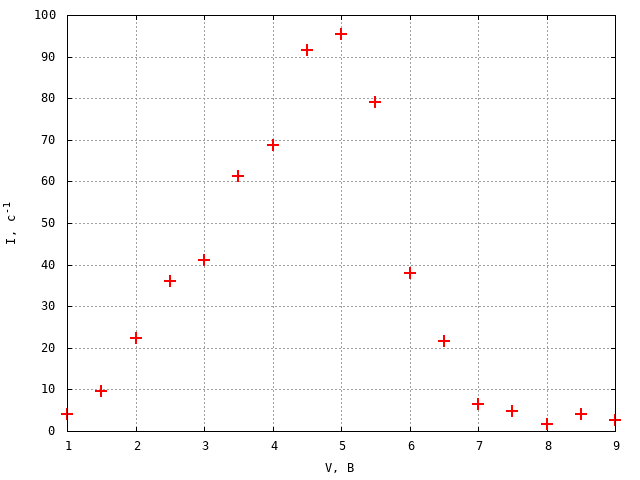
\includegraphics[width = 12cm, height=8cm]{plot1.png}
	\caption{Спектр источника}
\end{figure}
\par
	Заметим, что $23.8$ кэВ соответствует 5 В. Выберем значения порогов
\begin{align*}
	U_\text{нижн} &= 1 \, \text{В} \\
	U_\text{верх} &= 7 \, \text{В} \\ 
\end{align*}

\section*{Регистрация мёссбауэровского спектра}
\par
	Проведём регистрацию мёссбауэровского спектра для различных образцов.
\newpage
\subsection*{Образец 1}
	\begin{figure}[h!]
	\centering
	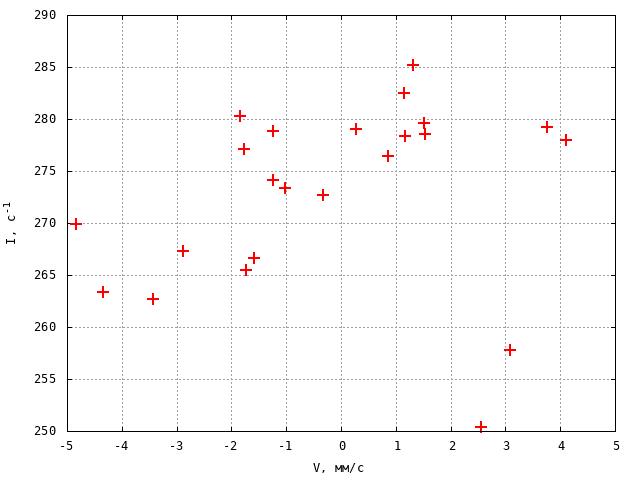
\includegraphics[width = 10cm, height=6cm]{plot2.png}
	\caption{Мёссбауэровский спектр для образца 1}
\end{figure}
\par
	\begin{table}[h!]
		\centering
		\begin{tabular}{|c|c|c|c|}
		\hline
			$\text{Г}_\text{эксп}$, мм/с & $\text{Г}_\text{эксп} \cdot 10^{-8}$, эВ & $\Delta E \cdot 10^{-8}$, эВ & $v_p$, мм/с \\
		\hline
			1.6 & 12.7 & 19.2 & 2.4 \\
		\hline
		\end{tabular}
	\end{table}
\subsection*{Образец 4}
	\begin{figure}[h!]
	\centering
	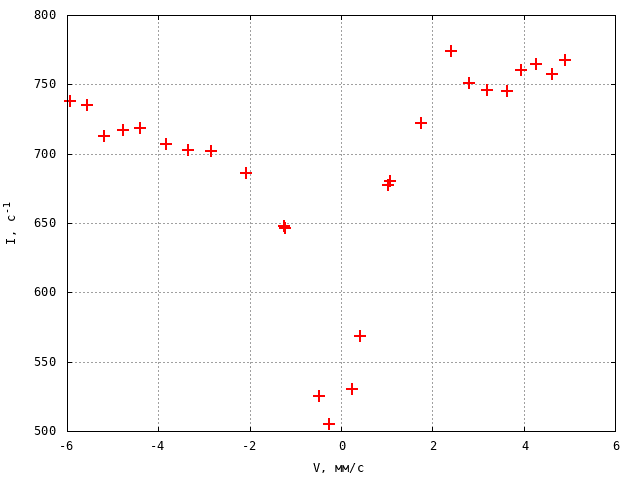
\includegraphics[width = 10cm, height=6cm]{plot3.png}
	\caption{Мёссбауэровский спектр для образца 4}
\end{figure}
\newpage
\par
	\begin{table}[h!]
		\centering
		\begin{tabular}{|c|c|c|c|}
		\hline
			$\text{Г}_\text{эксп}$, мм/с & $\text{Г}_\text{эксп} \cdot 10^{-8}$, эВ & $\Delta E \cdot 10^{-8}$, эВ & $v_p$, мм/с \\
		\hline
			2.3 & 18.2 & 0 & 0 \\
		\hline
		\end{tabular}
	\end{table}
\subsection*{Образец 2}
	\begin{figure}[h!]
	\centering
	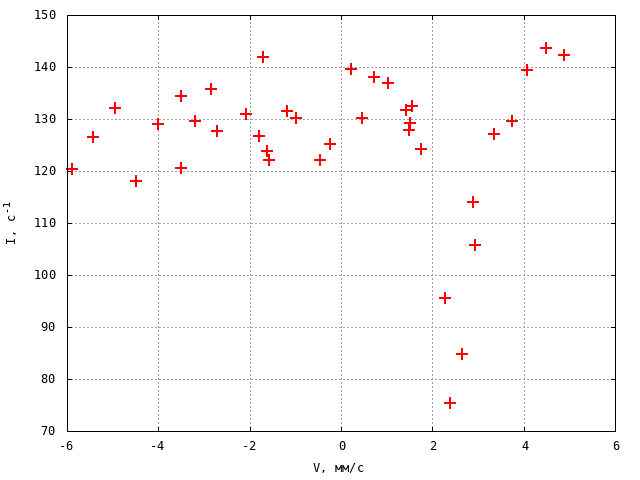
\includegraphics[width = 10cm, height=6cm]{plot4.png}
	\caption{Мёссбауэровский спектр для образца 2}
\end{figure}
\par
	\begin{table}[h!]
		\centering
		\begin{tabular}{|c|c|c|c|}
		\hline
			$\text{Г}_\text{эксп}$, мм/с & $\text{Г}_\text{эксп} \cdot 10^{-8}$, эВ & $\Delta E \cdot 10^{-8}$, эВ & $v_p$, мм/с \\
		\hline
			1.1 & 8.7 & 17.6 & 2.2 \\
		\hline
		\end{tabular}
	\end{table}
\end{document}

